\chapter{Introducción}\label{chap:Introduccion}
El objetivo principal de este trabajo de fin de grado (TFG) es mejorar la funcionalidad de VisualHFSM, una herramienta ya existente dentro de la plataforma JdeRobot\footnote{\url{http://jderobot.org}}\cite{peredadocencia, canas2013recent}, con la intención de conseguir una versión robusta y cómoda de utilizar que facilite la depuración de sus componentes, que finalmente pueda ser utilizada por terceros. En esta memoria haremos una pequeña introducción sobre la motivación para utilizar esta herramienta, los objetivos que nos hemos propuesto y los principales problemas a los que nos hemos tenido que enfrentar para conseguirlos. Además, explicaremos el estado en el que se encontraba anteriormente VisualHFSM y los cambios que ha sufrido durante sus distintas versiones, así como los cambios más significativos que vienen de la mano de esta nueva versión, que comentaremos en mayor detalle, ofreciendo una visión de cómo ha quedado finalmente esta herramienta. \\

A continuación, en este primer capítulo de introducción, hablaremos un poco sobre la robótica, situándola brevemente en la sociedad e industria actual, así como comentando las posibilidades que ofrecerá en un futuro, de los principales métodos utilizados para dotar a los robots de inteligencia, centrándonos en la programación visual y los autómatas de estado finito, y, por último, hablaremos de las características de VisualHFSM y de los cambios que ha experimentado en sus diferentes versiones, hasta llegar a su versión inmediatamente anterior a la expuesta en este TFG. \\

%%%%%%%%%%%%%%% Robótica %%%%%%%%%%%%%%%
\section{Robótica}
Coincidiendo con la explicación ofrecida en \cite{salamanques2012}, la robótica es la disciplina que se encarga del diseño, la construcción y la programación de los robots, y en ella se combinan diferentes disciplinas como la mecánica, la electrónica, la informática, la inteligencia artificial o la ingeniería del control, entre otras. Robot Industriesl Association (RIA) define el término robot como: \\

\begin{center}
``\textit{Un dispositivo multifuncional y reprogramable, diseñado para manipular y/o transportar material mediante movimientos programados para la ejecución de tareas diversas.}''\\
\end{center}

Además, un robot también puede definirse como toda aquella máquina o sistema informático dotado de sensores para obtener información del mundo que le rodea, actuadores que interactúan con el entorno y uno o más computadores. Dichos computadores ejecutan el software, el cual analiza la información recogida por los sensores y en función de ésta, envían las órdenes correspondientes, en forma de señales, a los actuadores, adaptándose así a diversas situaciones. A pesar de que el software no es un elemento físico, es precisamente en él donde reside toda la inteligencia del robot. \\

Adicionalmente, suele utilizarse como sinónimo de robot la palabra “autómata”, que puede definirse como:

\begin{center}
``\textit{Máquina automática programable capaz de realizar determinadas operaciones de manera autónoma y sustituir a los seres humanos en algunas tareas, en especial las pesadas, repetitivas o peligrosas. Puede estar dotada de sensores que le permiten adaptarse a las nuevas situaciones.}''
\end{center}

Aunque el término robot lleva presente en ciencia ficción desde mucho antes, es en la década de los ’50 cuando se desarrollan los primeros robots comerciales. Más concretamente, las primeras patentes aparecieron en 1946 con robots muy primitivos para el traslado de maquinaria de George Devol, coincidiendo con la aparición de las primeras computadoras. En 1954, Devol y Joseph Engelberger diseñaron el primer robot programable, que acuñó el término \textit{autómata universal}, posteriormente recortado a \textit{Unimate}. Este robot fue instalado por primera vez en 1961 en la Ford Motors Company, para atender una máquina de fundición de troquel. Podemos observar una imagen de este robot en la figura \ref{fig:unimate}. Con esto empezó la participación de los robots en uno de los principales usos a los que estas máquinas han estado destinadas hasta la actualidad: las tareas industriales.  \\

Con el paso del tiempo, los robots fueron irrumpiendo con mayor fuerza cada vez para realizar tareas sucias, peligrosas, difíciles o extremadamente repetitivas para ser realizadas por un ser humano, cobrando una especial importancia en las cadenas de montaje, donde por ejemplo, en el caso de la industria automovilística, el proceso se encuentra altamente automatizado, con robots que se encargan desde tareas como soldar el chasis hasta pintar la carrocería, pasando por tareas de logística relacionadas con el servicio y transporte de piezas por los almacenes. Un ejemplo de lo automatizado que está todo este proceso se ve en la figura \ref{fig:robotsCars}. \\

\begin{figure}[htbp]
	\begin{subfigure}{0.45\textwidth}
	\centering	
	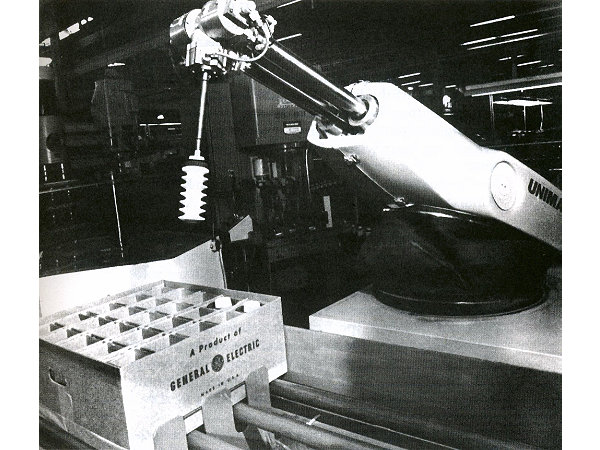
\includegraphics[height=4cm]{imgs/1_introduction/unimate.jpeg}
	\caption{Robot Unimate}
	\label{fig:unimate}
	\end{subfigure}
	\hfill
	\begin{subfigure}{0.45\textwidth}
	\centering	
	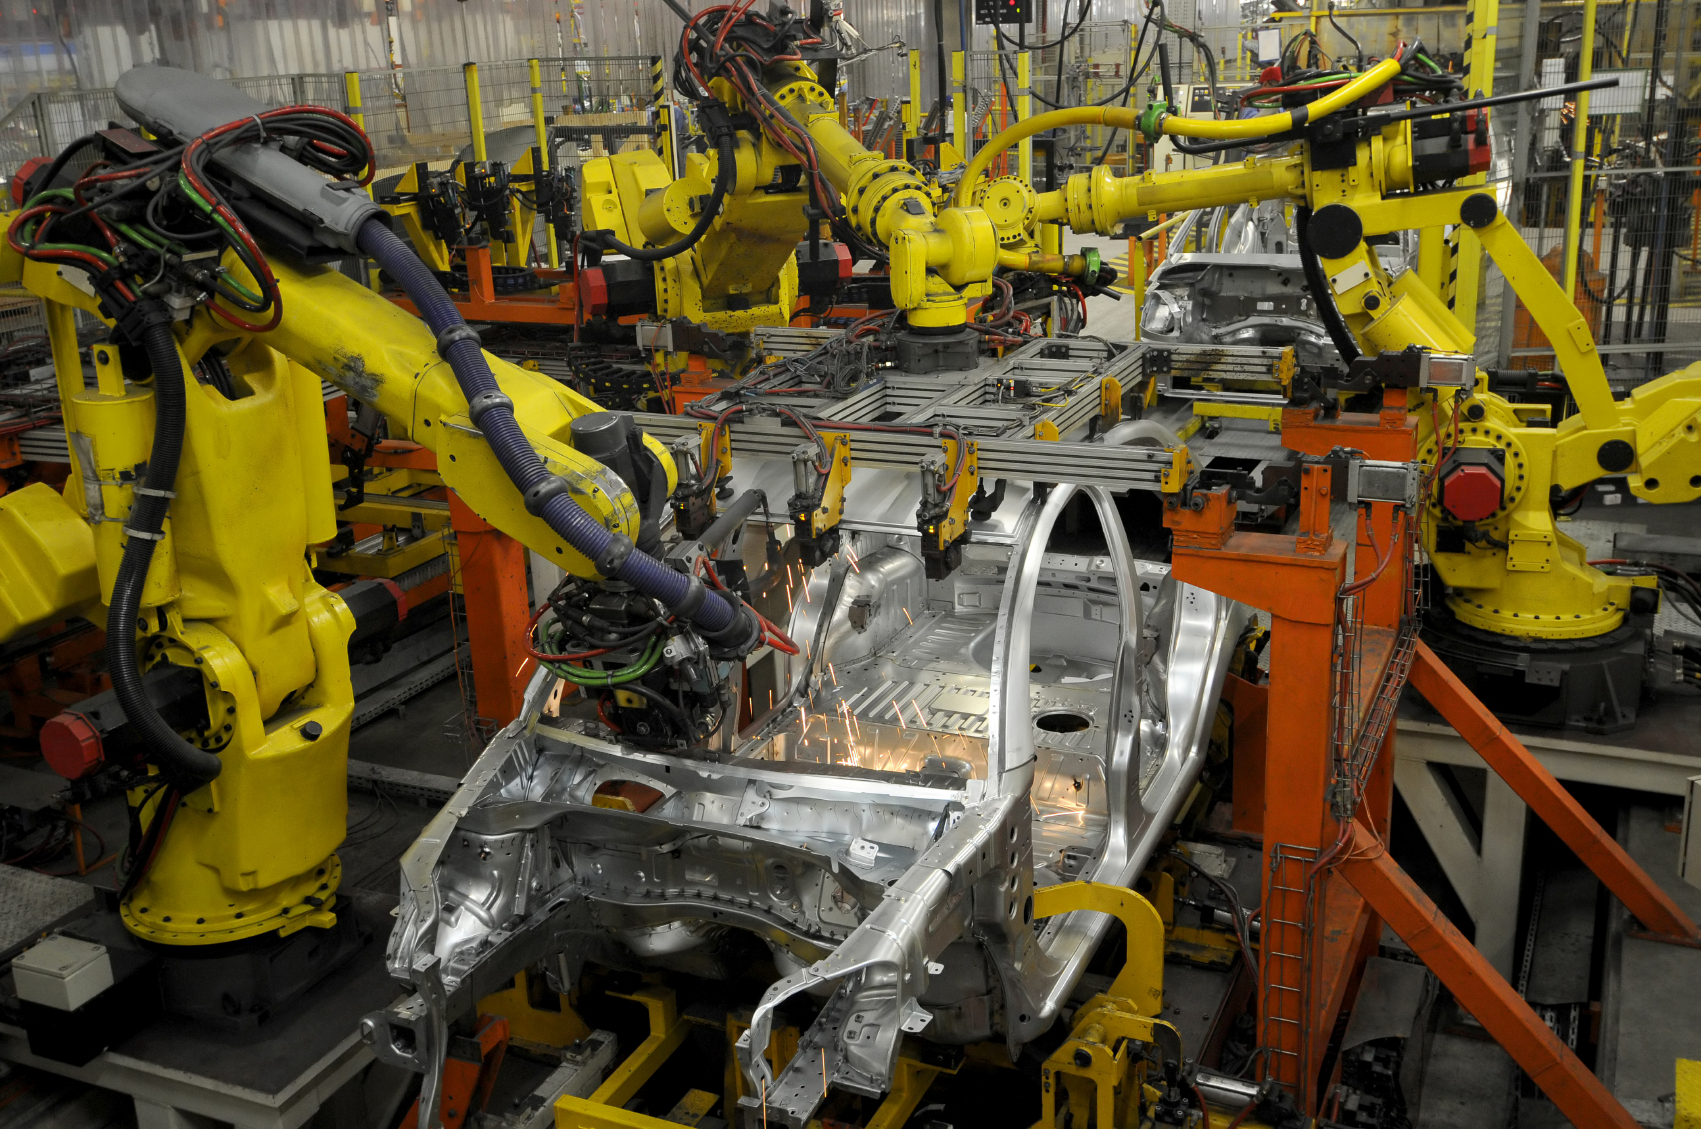
\includegraphics[height=4cm]{imgs/1_introduction/robotsCars.jpg}
	\caption{Brazos robóticos montando coches.}
	\label{fig:robotsCars}
	\end{subfigure}
\caption{Aplicaciones de robots en la industria.}
\end{figure}

Otra muestra del uso cada vez más común en la industria es el embalaje de productos, como sucede en el caso de la empresa ABB\footnote{\url{http://www.abb.es}}, dónde unos brazos robóticos dotados de visión son capaces de organizar y colocar distintos tipos de productos que van pasando delante de ellos por una cinta transportadora. \\

Otro ejemplo de aplicaciones para robots es la empresa Kiva Systems\footnote{\url{http://www.kivasystems.com}}, recientemente comprada por Amazon, el gran gigante de la venta de productos por internet. En esta empresa tienen robots encargados de mover y reubicar estanterías de varios pisos de alturas llenas de paquetes. Realizan esta tarea de manera completamente autónoma y son, además, capaces de coordinarse entre ellos para elegir la manera más óptima de realizar estos movimientos, ahorrando así una gran cantidad de recursos en la tarea (figura \ref{fig:amazonRobots}). 
	
\begin{figure}[htbp]
	\centering
	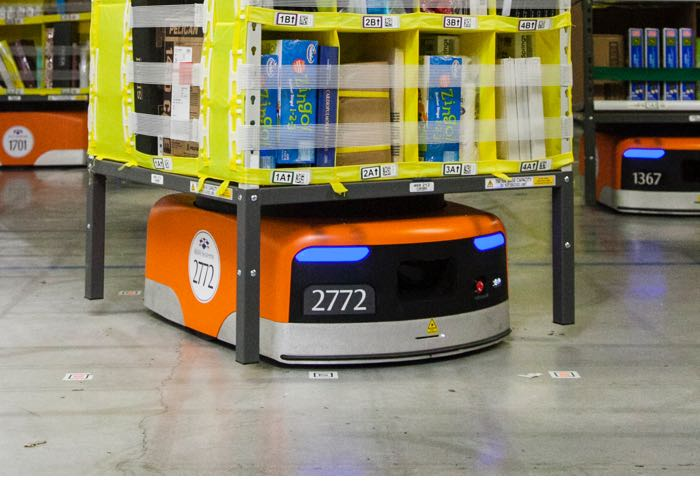
\includegraphics[height=5cm]{imgs/1_introduction/robotsAmazon.jpg}
	\caption{Robots de Amazon.}
	\label{fig:amazonRobots}
\end{figure}
	
Pero los robots no se limitan a realizar tareas industriales. También aparecen realizando actividades como limpieza de residuos tóxicos, localización y desactivación de explosivos (figura \ref{fig:robotExplosives}), búsqueda y rescate de personas, exploración de volcanes activos o fondos marinos (figura \ref{fig:robotSea}), por citar algunos ejemplos. También presentan un uso muy destacado en la exploración espacial, donde multitud de distintos robots han aportado la posibilidad de realizar misiones como la exploración de Marte mediante las sondas gemelas Spirit y Opportunity, o la construcción y mantenimiento de la ISS o EES (Estación Espacial Internacional) gracias al complejo brazo robótico ERA. \\

Otro de los campos donde el uso de robots se está haciendo cada vez más popular es la medicina, especialmente en la cirugía laparoscópica, que busca realizar las mínimas incisiones posibles. Actualmente empieza a emplearse equipamiento robótico teledirigido que permita a los cirujanos realizar operaciones muy delicadas, como por ejemplo de cirugía ocular o neurocirugía, con una precisión altísima y sin temor a que el pulso les tiemble. También se emplean robots en los laboratorios médicos para poder manejar sustancias biológicas potencialmente dañinas con el mínimo riesgo. Un claro ejemplo de estos robots es el robot "Da Vinci", creado por la empresa norteamericana Intuitive Surgical \footnote{\url{http://www.intuitivesurgical.com/}} y aprobado en el año 2000. Este sistema quirúrjico es teleoperado y se usa en múltiples procedimientos quirúrjicos con la idea de conseguir un enfoque mínimamente invasivo. Este robot puede verse en la figura \ref{fig:davinci}. \\

Observando esta gran expansión que está experimentando la robótica en campos tan diversos, no es de extrañar que actualmente también podamos encontrar robots domésticos al alcance de cualquiera. El caso más común en este ámbito es el de los robots aspiradora, actualmente comercializados por multitud de empresas, capaces de ser manejados por cualquier tipo de persona, y que gracias a sus comportamientos autónomos son capaces de limpiar pisos enteros sin necesidad de ser programados por el usuario final. Y aprovechando que hablamos de robots más económicos al alcance de todos, merece la pena mencionar que también han surgido otro tipo de robots, destinados a la generalidad del público con el fin de proporcionar entretenimiento: los robots de ocio. En los últimos años han surgido varios productos consistentes en robots que aunque técnicamente son muy avanzados si nos fijamos en los estándares de hace tan solo 30 años, no son más que “juguetes” para gran parte de la población actual. Este es el caso del robot mascota de Sony, el Robot Aibo, o el Ev3 de Lego (figura \ref{fig:ev3Lego}), un “juguete” que permite construir, programar y controlar tus propios robots. \\

\begin{figure}[htbp]
	\begin{subfigure}{0.45\textwidth}
	\centering
	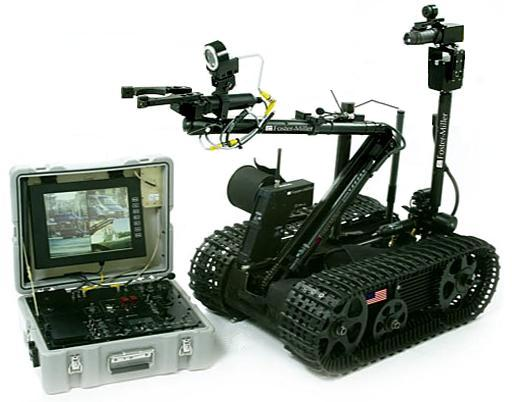
\includegraphics[height=3cm]{imgs/1_introduction/robotExplosives.jpg}
	\caption{Robot artificiero teleoperado.}
	\label{fig:robotExplosives}
	\end{subfigure}
	\hfill
	\begin{subfigure}{0.45\textwidth}
	\centering
	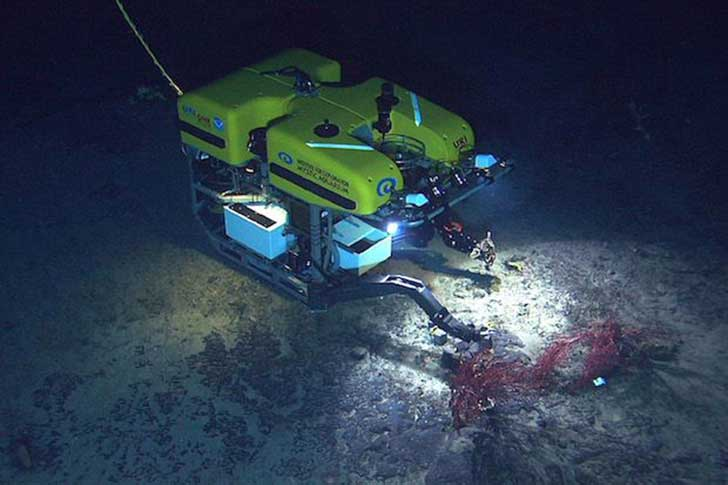
\includegraphics[height=3cm]{imgs/1_introduction/robotSea.jpg}
	\caption{Robot explorador de fondos marinos.}
	\label{fig:robotSea}
	\end{subfigure}
	\hfill
	\begin{subfigure}{0.45\textwidth}
	\centering
	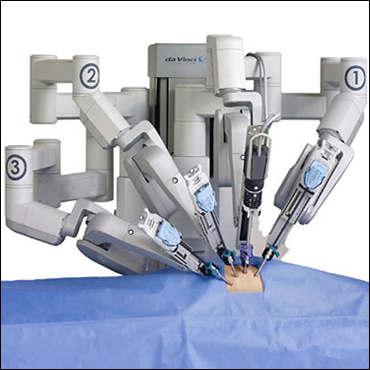
\includegraphics[height=3cm]{imgs/1_introduction/davinci.jpg}
	\caption{Robot cirujano Da Vinciteleoperado.}
	\label{fig:davinci}
	\end{subfigure}
	\hfill
	\begin{subfigure}{0.45\textwidth}
	\centering
	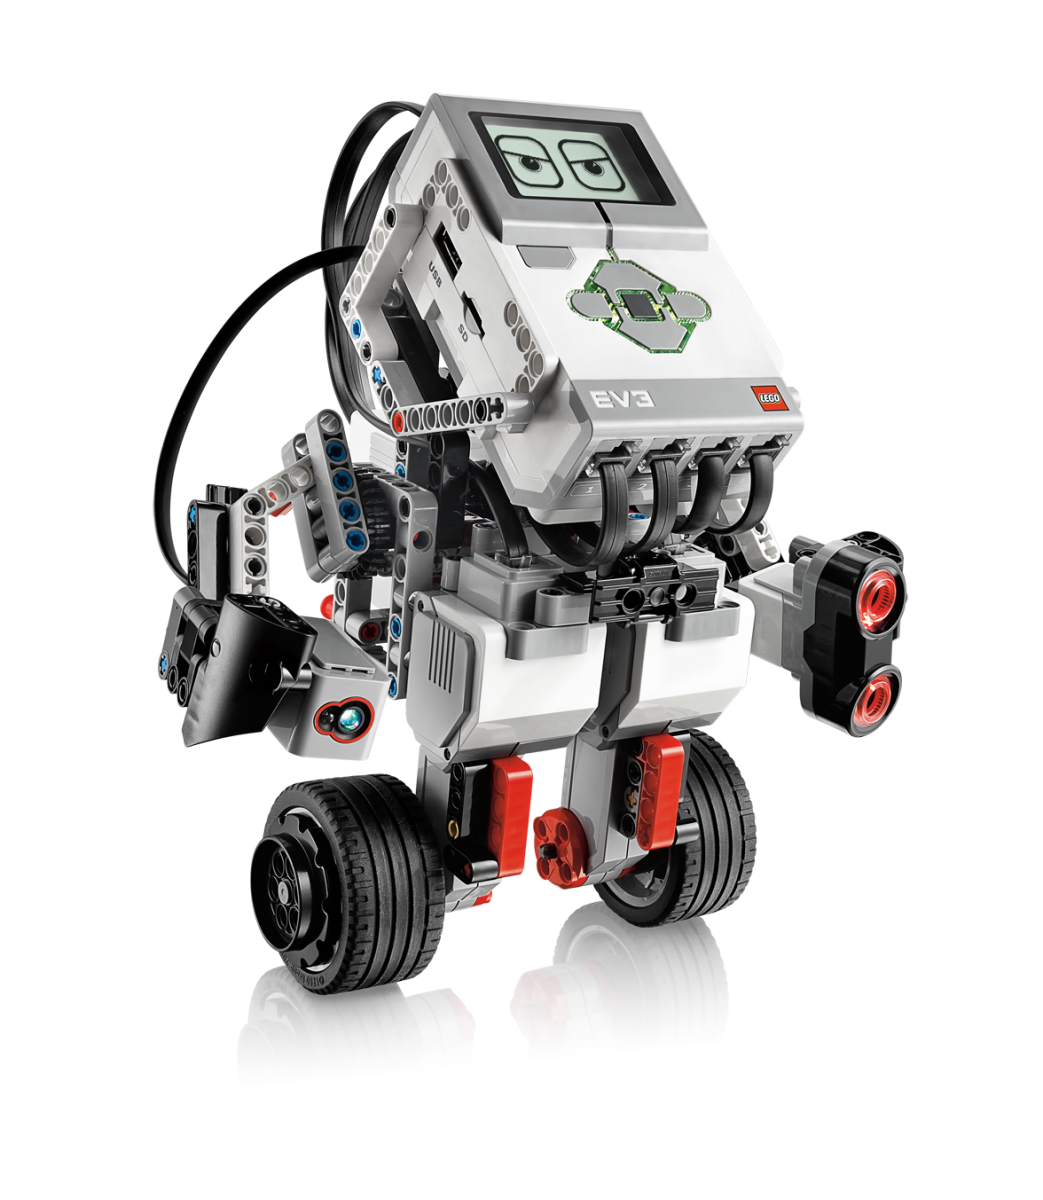
\includegraphics[height=3cm]{imgs/1_introduction/ev3Lego.png}
	\caption{Ev3 de Lego.}
	\label{fig:ev3Lego}
	\end{subfigure}
\caption{Aplicaciones de robots fuera de la industria.}
\end{figure}

Otra aplicación cada vez más extendida es el uso de UAVs (Unmanned Aerial Vehicle o vehículo aéreo no tripulado), o más comúnmente conocidos como drones. En Alemania usan este tipo de robots para vigilar los trenes, protegiéndolos así de grafiteros y vándalos. Con esta medida están ahorrar dinero, pues se estima en 10 millones de dólares anuales el gasto que supone limpiar los grafitis. Actualmente, en la Comunidad de Madrid, se está estudiando el uso de robots de este estilo, equipados con cámaras y sensores que detectan gases y agentes radiactivos, para ayudar a los servicios de emergencia en labores de rescate, reduciendo así no sólo costes económicos, sino también riesgos humanos. Además, en España, Endesa ha desplegado 14 drones equipados con cámaras de alta resolución y termográficas para revisar las líneas eléctricas. También la empresa Amazon, de la que ya hemos hablado anteriormente, ha comunicado recientemente que quiere usar drones para hacer repartos a domicilio de sus productos, llevando así el paquete hasta el comprador en el mismo día en el que éste adquirió el producto. También se está haciendo especialmente popular el uso de drones para la agricultura de precisión, dado que facilitan a los agricultores la capacidad de observar sus campos desde el aire, permitiéndoles observar las incidencias en cada campaña agrícola, ofreciendo información sobre el estado hídrico, el grado de desarrollo vegetativo y su estado sanitario en tiempo real. Ofrecen también la posibilidad de realizar riegos, fertilizaciones o tratamientos sanitarios en las zonas que los necesiten en función a la información recogida. En la figura \ref{fig:agriculturaPrecision} se puede observar un drone utilizado en este campo. Sin embargo, existen todavía muchas más aplicaciones en las que estos robots resultan útiles, como la prevención y el control de incendios, para fotografía, vídeo y cartografía aérea, buscar personas desaparecidas, etc.

\begin{figure}[htbp]
	\begin{subfigure}{0.45\textwidth}
	\centering
	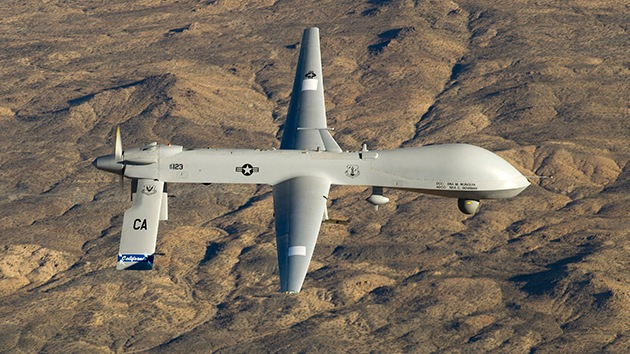
\includegraphics[height=4cm]{imgs/1_introduction/uav.jpg}
	\caption{Drone militar.}
	\label{fig:militarDrone}
	\end{subfigure}
	\hfill
	\begin{subfigure}{0.45\textwidth}
	\centering
	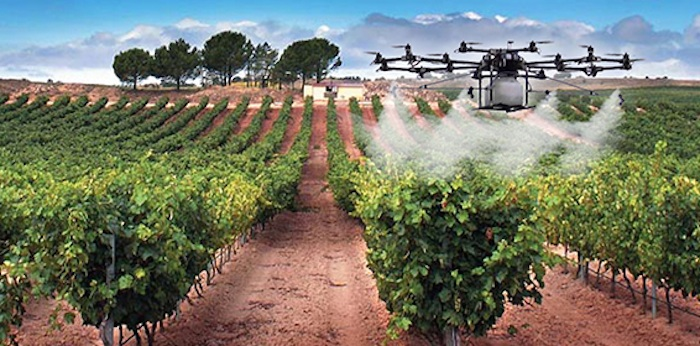
\includegraphics[height=4cm]{imgs/1_introduction/agriculturaPrecision.jpg}
	\caption{Drone en la agricultura de precisión.}
	\label{fig:agriculturaPrecision}
	\end{subfigure}
\caption{Distintos ejemplos de drones.}
\end{figure}

Otro área que se ha beneficiado de los avances de la róbotica es la industría del automóvil. Uno de los ejemplos más habituales de esta influencia son los sistemas de aparcamiento autónomo (figura \ref{fig:autoParking}), y es que cada vez son más los coches que ofrecen la posibilidad de aparcar con sólo pulsar un botón. Sin embargo, hay ejemplos más sofisticados de esta influencia, como los Model S de Tesla, que puede observarse en la figura \ref{fig:modelS}. Estos vehículos disponen de una actualización que les dotará de una función de piloto asistido y casi-automático que permitirá al conductor relajarse un rato durante las horas de más tráfico. Aunque estos coches no serán capaces de llegar autónomamente de un sitio A a otro B, son capaces de circular por la calle en la que se encuentran por si solos. Con esto nos acercamos al auténtico objetivo que se persigue con estra mezcla de robots y vehículos: los coches autónomos. Se trata de vehículos dotados de sensores e inteligencia suficiente como para conducirse por sí mismos. Aunque esta tecnología aún no está disponible, está sufriendo un gran desarrollo y una fuerte investigación y apoyo por parte de diversos sectores, destacando el fuerte impulso otorgado por Google. \\

\begin{figure}[htbp]
	\centering
	\begin{subfigure}{0.45\textwidth}
	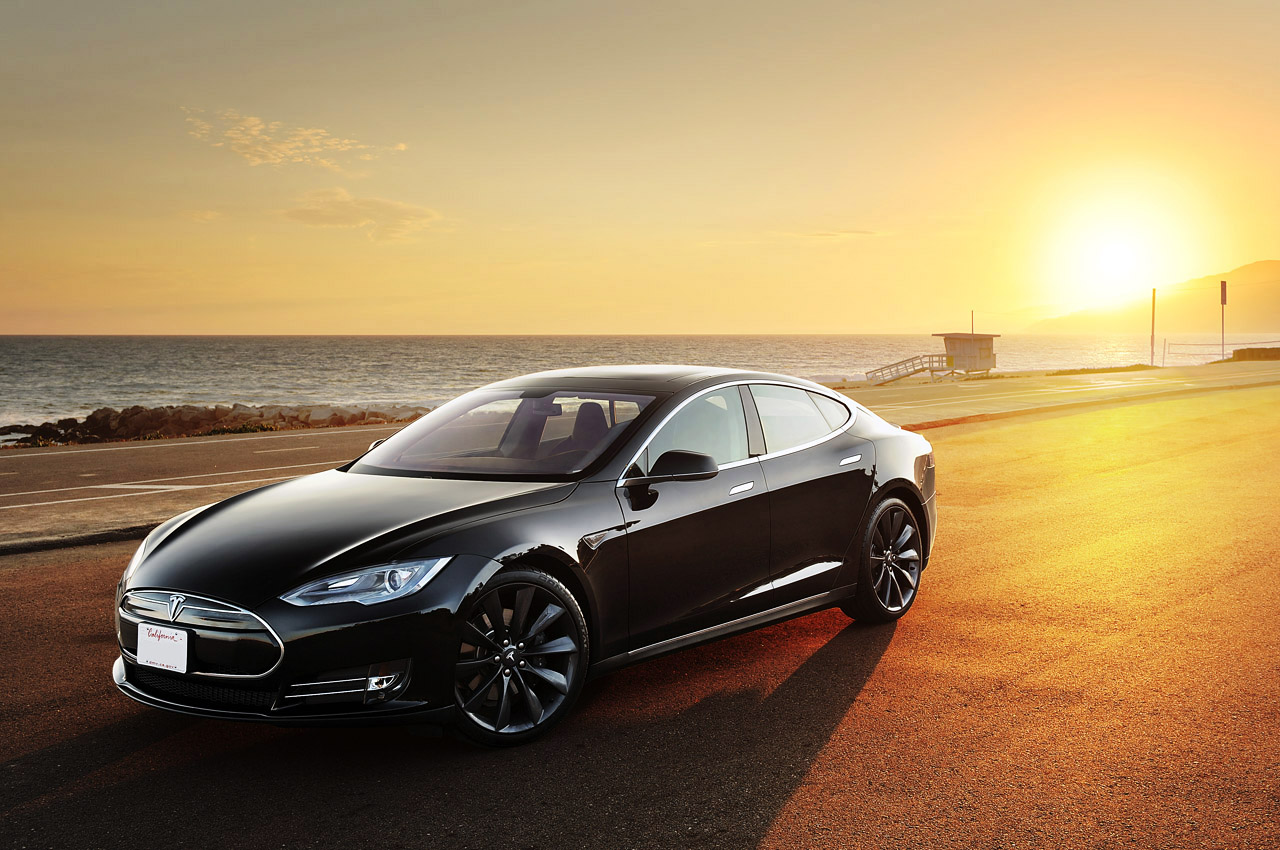
\includegraphics[height=4cm]{imgs/1_introduction/modelS.jpg}
	\caption{Model S deTesla.}
	\label{fig:modelS}
	\end{subfigure}
	\hfill
	\centering
	\begin{subfigure}{0.45\textwidth}
	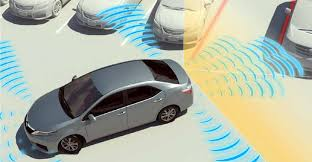
\includegraphics[height=4cm]{imgs/1_introduction/autoparking.jpeg}
	\caption{Aparcamiento autónomo.}
	\label{fig:autoParking}
	\end{subfigure}
\caption{Avances robóticos en automóviles.}
\end{figure}



En resumen, la robótica es un campo que ha sufrido una gran evolución en los últimos años, pero que aún puede evolucionar mucho más. Cada vez son más las aplicaciones comerciales robóticas, y esta tendencia continúa intensificándose. Se trata, por lo tanto, de un sector con una gran perspectiva de futuro y casi ilimitadas posibilidades y aplicaciones, que van aumentando a la vez que aumenta nuestra tecnología actual.

%%%%%%%%%%%%%%% Programación en robots %%%%%%%%%%%%%%%
\section{Programación en robots}
Ya hemos comentado el gran desarrollo que han sufrido los robots en una gran variedad de campos. Este desarrollo se debe en gran medida a su inteligencia, que no reside en los sensores encargados de captar la información del exterior o del interior propio robot, si no que radica en su software. El software es el encargado de decidir qué debe hacerse en función de toda la información que han recogido los distintos sensores. Al igual que nuestro cerebro, el software de los robots es el encargado de analizar las diversas situaciones que se le presenten, y dar una respuesta, activando los actuadores correspondientes para reaccionar de la forma más conveniente posible. La funcionalidad del robot reside fundamentalmente en su programación, en el software que maneja los recursos hardware como los sensores y actuadores.

\subsection{Plataformas}
Aunque la inteligencia de los robots reside en su software, su programación no es sencilla, principalmente debido a que no existe una metodología universal estandarizada para programar robots. Históricamente, lo único que se utilizaban eran los \textit{drivers} proporcionados por su fabricante, siendo el sistema operativo casi inexistente, consistente únicamente en una colección de \textit{drivers} con rutinas para leer valores de los sensores y escribir valores en los actuadores. Esta forma de programar se refleja en la figura \ref{fig:onDrivers}.

\begin{figure}[htbp]
	\begin{subfigure}{0.45\textwidth}
	\centering
	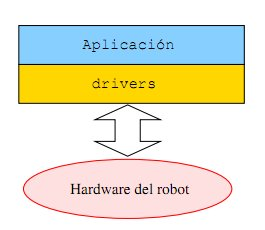
\includegraphics[height=5cm]{imgs/1_introduction/progRobots1.jpg}
	\caption{Sobre drivers de sensores y actuadores}
	\label{fig:onDrivers}
	\end{subfigure}
	\hfill
	\begin{subfigure}{0.45\textwidth}
	\centering
	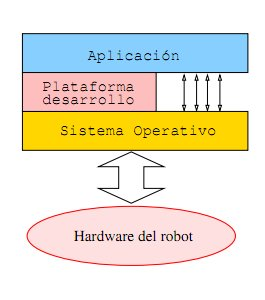
\includegraphics[height=5cm]{imgs/1_introduction/progRobots2.jpg}
	\caption{Sobre una plataforma.}
	\label{fig:onPlatform}
	\end{subfigure}
\caption{Distintos esquemas de programación de robots.}
\end{figure}

El principal problema de esta forma de desarrollar software es que resulta complicada, costosa, y, sobre todo, muy poco reutilizable. Es por esto que se hizo necesario que el desarrollo del software empezara a simplificarse, añadiendo una capa entre el sistema operativo y las aplicaciones robóticas: las plataformas de desarrollo (figura \ref{fig:onPlatform}). Añadiendo esta capa se consigue un acceso más sencillo y estandarizado a los sensores y actuadores, haciendo que a la aplicación robótica no le importe si el sensor láser que tiene el robot tiene unas características específicas u otras, ya que le ofrecerá la información en el mismo modo. \\

En los últimos años la comunidad robótica ha empezado a aplicar conceptos y metodologías de la ingeniería del software a este campo, haciendo un mayor énfasis en la reutilización del código, diseños de software distribuido, etc., y han aparecido varias plataformas de desarrollo de aplicaciones, siendo sus principales características las siguientes:

\begin{itemize}
\item Proveen de una capa de acceso al hardware (HAL, por sus siglas en inglés \textit{Hardware Access Layer}) más o menos portable.
\item Ofrecen una arquitectura de software concreta a las aplicaciones.
\item Incluyen herramientas y bibliotecas con funcionalidad lista para ser utilizada.
\end{itemize}

Muchas de estas plataformas surgidas en los últimos años estás orientadas a componentes. Son sistemas conformados en diferentes componentes lógicos o funcionales con interfaces que se usan para la comunicación entre dichos componentes. Entre estas plataformas se pueden destacar \emph{ROS}\footnote{\url{http://www.ros.org/}} (Quigley et al., 2009), \emph{Orca}  (Brooks et al., 2007, Makarenko et al., 2006), \emph{Microsoft Robotics Studio}, \emph{RoboComp} y \emph{JdeRobot} (Cañas Plaza, 2003), entre otras.

\subsection{Lenguajes Visuales}
Como se explica en \cite{borja2014}, existen también diferentes formas de programar un robot. La primera de ellas consiste en escribir directamente su código fuente, pudiendo utilizarse lenguajes como Java, C/C++ o Python, entre otros, igual que en la programación de cualquier otra aplicación informática. Lo que hace que un lenguaje pueda ser usado para programar robots son las bibliotecas que estén desarrolladas para él. \\

A parte de estos lenguajes “tradicionales” de programación, ha habido intentos de crear lenguajes específicos para programar robots que contasen con primitivas propias de la robótica. En este tipo de lenguajes se encuentran los \textit{Taks Descrition Language} (TDL) o \textit{Reaction Active Packages} (RAP). Pero lo que realmente se puede considerar un avance en la programación específica es el surgimiento de los \emph{lenguajes de programación visual} (LPV). Estos lenguajes se caracterizan por utilizar únicamente elementos gráficos para programar, de forma que no es necesario introducir código escrito “a mano”, como se hace tradicionalmente. Este tipo de lenguajes ofrecen una programación muy intuitiva y didáctica, pudiéndose observar además de manera muy clara  aspectos esenciales en un programa informático, como el flujo de ejecución, sus condiciones, bucles, etc. En resumen, podríamos definir un LPV como:

\begin{itemize}
\item Un lenguaje de programación que utiliza una representación visual como gráficos, dibujos, iconos o animaciones.
\item Un lenguaje que manipula información visual o soporta interacción visual, o permite programar utilizando expresiones visuales.
\item Un conjunto de símbolos de texto y gráficos con una interpretación semántica que es utilizada para comunicar acciones en un entorno.
\item Lenguaje de programación donde se usan técnicas visuales para expresar relaciones o transformaciones en la información.
\end{itemize}

Hay que aclarar que un LPV no es un entorno integrado de desarrollo (IDE). La diferencia es que un LPV debe ser capaz de llevar a cabo todas las tareas de programación de forma visual, sin tener que recurrir a la representación textual. \\

Entonces, ¿por qué insistimos en comunicarnos con los ordenadores y las máquinas mediante lenguajes de programación textuales? ¿No sería mejor hacerlo mediante una programación que aproveche nuestra naturaleza visual? Los autores de los LPV discuten que la respuesta a esta pregunta es sí, siendo algunas de las principales motivaciones:

\begin{itemize}
\item Mucha gente piensa y recuerda cosas en términos de esquemas y cuadrados.
\item Las personas nos relacionamos con el mundo de forma intrínsecamente gráfica y utilizamos imágenes como el componente primario del pensamiento creativo.
\end{itemize}

Sin embargo, los LPV también presentan algunas limitaciones, siendo la más importante que, al no poder introducir código textualmente, el programador se encuentra limitado a utilizar los recursos que éste le brinde. \\

Un ejemplo muy ilustrativo de LPV en robótica es el lenguaje RCX de Lego. Fue creado inicialmente para niños, caracterizándose por su simplicidad y legibilidad. Se empleó para la programación de su juguete RCX, siendo utilizado más tarde también en su evolución, el NXT. Estaba pensado para poder ser utilizado por niños, y consta de bloques visuales que representan acciones o condiciones, permitiendo, mediante el apilamiento de dichos bloques, componer un comportamiento más o menos complejo de  manera sencilla. Mediante estos bloques puede lograrse que el robot se mueva, emita un sonido, o reaccione a distintos eventos. En la figura \ref{fig:lego} se puede ver el aspecto de este lenguaje.

\begin{figure}[htbp]
	\centering
	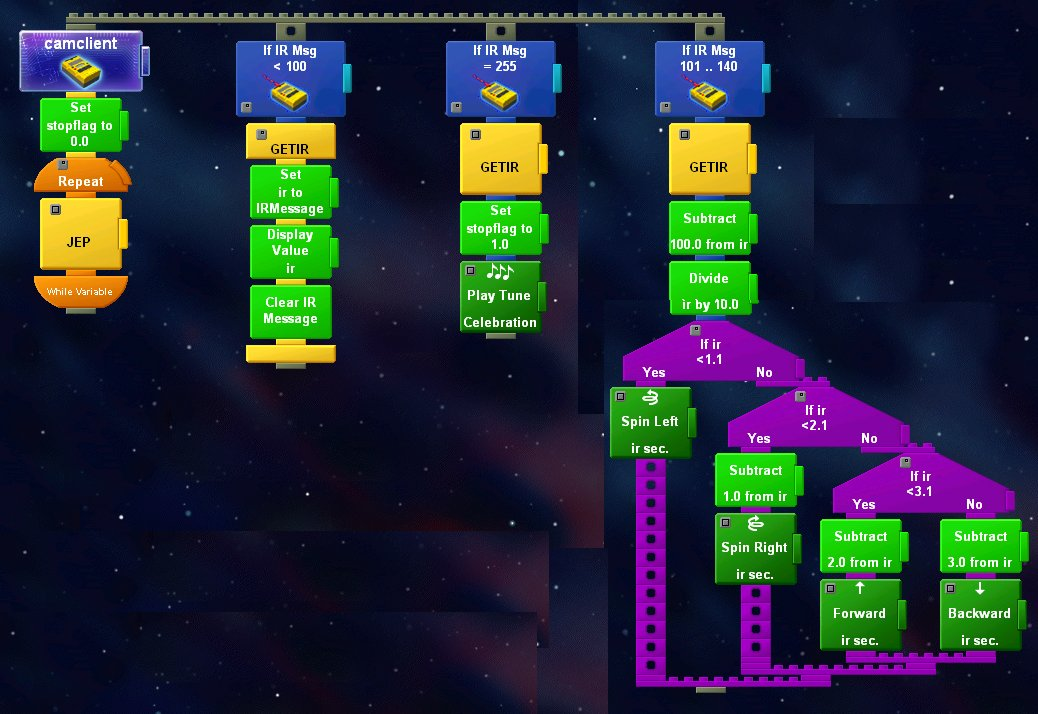
\includegraphics[height=6cm]{imgs/1_introduction/rcxCode.jpg}
	\caption{Imagen RCX code de Lego.}
	\label{fig:lego}	
\end{figure}

Otro de los puntos fuertes de los LPV es que, gracias a su aspecto fácilmente legible, se convierten en elementos didácticos ideales, permitiendo así un primer y sencillo contacto para los niños con el mundo de la programación. Aunque no tengan que escribir código directamente, estos lenguajes les permiten acostumbrarse y empezar a entender distintas estructuras empleadas en la programación, como los condicionales o los bucles, entres otros. Precisamente dentro de este enfoque entran los dos ejemplos que vamos a citar a continuación: \emph{Scratch} y \emph{Blockly}. \\

\emph{Scratch}\footnote{\url{https://scratch.mit.edu/}}\cite{scratchEducativo} es un lenguaje pensado para que los pequeños aprendan a pensar de forma creativa, razonar de forma sistemática, y además, tengan un primer contacto con la programación. Este lenguaje permite programar historias interactivas, juegos, animaciones, y compartirlos con los demás en la comunidad online. Y, por supuesto, toda la programación se realiza de forma visual, concatenando distintos bloques, tal y como podemos ver en la figura \ref{fig:scratch}. \\

\emph{Blockly}\footnote{\url{https://developers.google.com/blockly/}}\cite{learningWithBlockly} es una librería de JavaScript que también utiliza bloques para programar. Es un proyecto open source de Google similar a Scratch que apareció por primera vez en 2012. Esta librería está siendo ampliamente utilizada sobre todo para aplicaciones educativas como \textit{Blockly Games}\footnote{\url{https://blockly-games.appspot.com/?lang=es}}, pero no reduciéndose a este campo, dado que también está siendo utilizado como IDE para desarrollar aplicaciones para Android, entre otros usos. Si observamos la figura \ref{fig:blockly} podremos ver un ejemplo resuelto de uno de los distintos juegos educativos que se ha hecho con esta librería. \\

\begin{figure}[htbp]
	\centering
	\begin{subfigure}{0.49\textwidth}
	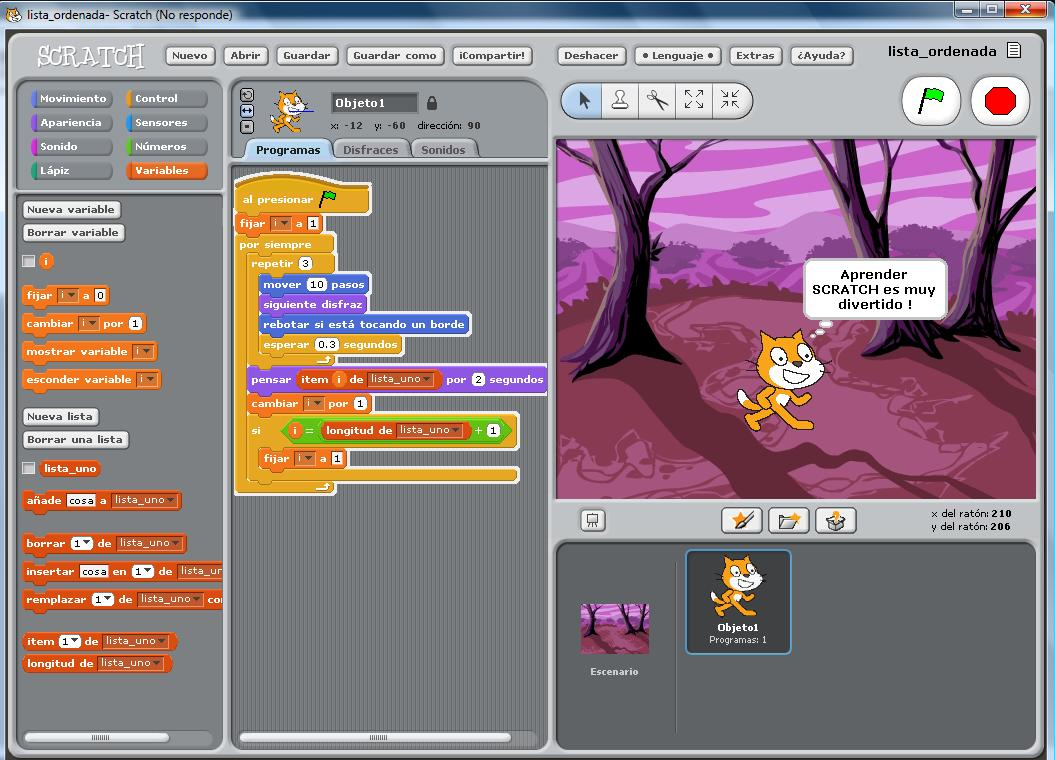
\includegraphics[height=6cm]{imgs/1_introduction/scratch.jpg}
	\caption{Ejemplo de uso de Scratch.}
	\label{fig:scratch}
	\end{subfigure}
	\hfill
	\centering
	\begin{subfigure}{0.49\textwidth}
	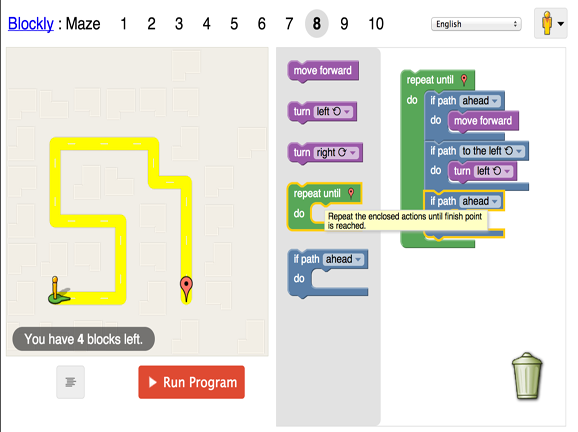
\includegraphics[height=6cm]{imgs/1_introduction/blockly.png}
	\caption{Ejemplo de uso de Blockly.}
	\label{fig:blockly}
	\end{subfigure}
\caption{Aplicaciones educativas de los LPV.}
\end{figure}

\subsection{Autómatas}
Los autómatas finitos o Máquinas de Estado Finito (FSM, \textit{Finite State Machines}) se han utilizado exitosamente para representar comportamientos de robots\cite{foukarakis2014combining}, representándolos de manera compacta y abstracta. Con estos autómatas el comportamiento es representado mediante un conjunto de \textit{estados}, cada uno de los cuales está encargado de realizar una tarea particular. El sistema puede cambiar de un estado a otro mediante \textit{transiciones}, que son las condiciones de cambio que dependen de ciertos eventos o cambios producidos en los sensores del robot, ya sean internos o externos. \\

Los autómatas de estados finitos ofrecen una forma inteligente y sencilla de organizar el código de control y de percepción dentro de un robot móvil. Han sido explorados en investigación y también incorporados en plataformas de desarrollo robóticas recientes, con herramientas que le dan al programador la capacidad de abstraerse un poco más de los detalles de la implementación y centrarse en la lógica del comportamiento que está interesado en programar. De esta forma, la mayor parte del código es autogenerado en base al comportamiento programado, lo que hace disminuir en gran medida la aparición de errores y reducir el tiempo de desarrollo de forma considerable, permitiendo, además, programar comportamientos complejos de forma robusta. \\

\begin{figure}
	\centering
	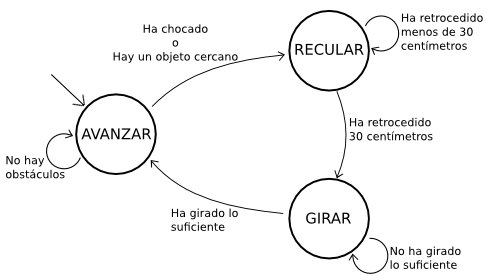
\includegraphics[height=5cm]{imgs/1_introduction/AutomataRobot.jpg}
	\caption{Ejemplo de autómata que define un comportamiento sencillo para un robot.}
	\label{fig:simpleAutomata}
\end{figure}

Conviene añadir también, que esta forma de representar el comportamiento de los robots utilizando autómatas de estado finito combina a la perfección con el uso de un LPV, o, al menos, con una aproximación más gráfica que los lenguajes de programación puramente textuales, dado que el flujo de control puede ser perfectamente representado gráficamente mediante un esquema de estados y transiciones, tal cómo hemos se ve en la figura \ref{fig:simpleAutomata}. \\

Una herramienta comercial que utiliza programación visual en base a autómatas jerárquicos es \textit{XaitControl}, de la empresa Xaitment, empleada en videojuegos para programar la inteligencia artificial de los jugadores automáticos. Como se aprecia en la figura \ref{fig:xaitControl}, este programa cuenta con una zona principal donde se pinta el autómata, una vista lateral que muestra toda la estructura creada, y otros paneles con distintas informaciones sobre procedimientos auxiliares, control de flujo de ejecución, etc.  Esta herramienta cuenta además con ciertas características muy avanzadas, como por ejemplo la capacidad de diseñar un autómata finito no determinista (AFND). Un AFND es un autómata en el que, por ejemplo, se pueda transitar por dos caminos diferentes entre un estado origen y un estado final. Permite también la creación de proyectos compuestos por uno o varios autómatas jerárquicos cada uno, pudiendo ver todas las dependencias existentes entre ellos gracias a la vista en forma de árbol. Cuenta con un compilador que le permite lanzar la aplicación programada, utilizando la misma interfaz para ver los progresos, pudiendo establecer puntos de parada en el flujo de ejecución, avance instrucción a instrucción y otras funcionalidades comunes a cualquier depurador. \\

\begin{figure}
	\centering
	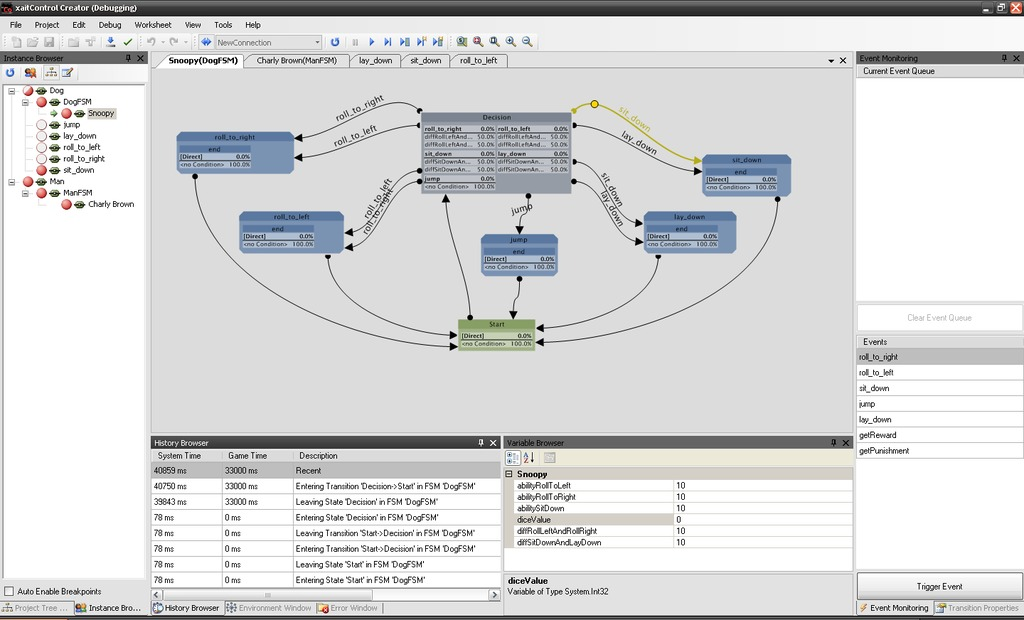
\includegraphics[height=5cm]{imgs/1_introduction/xaitControl.jpg}
	\caption{Captura de XaitControl.}
	\label{fig:xaitControl}
\end{figure}

Otra herramienta que utiliza esta aproximación de autómatas finitos es \textit{SMACH}\footnote{\url{http://www.ros.org/wiki/smach}}\cite{bohren2011towards, smach2013}, una herramienta de la plataforma ROS que consiste en una arquitectura a nivel de tarea que permite crear comportamientos complejos para robots de forma rápida. En su núcleo, SMACH es una librería de Python que permite construir máquinas de estado finito jerárquicas. Para esto, hay que escribir el código  necesario para crear y describir cada estado y transición, por lo que no puede considerarse un LPV, dado que la programación no se realiza de forma gráfica sino introduciendo el código. Sin embargo, esta librería viene también con el \textit{SMACH viewer} (figura \ref{fig:smach}), una herramienta que muestra la máquina de estados desarrollada en tiempo de ejecución, de forma que podemos ver el gráfico o la vista de árbol de nuestro autómata aunque no los dos a la vez. También muestra todos los estados y transiciones, así como aquellos que estén activos y una ventana de ayuda dónde se pueden ver los datos relativos a este estado activo. \\

\begin{figure}
	\centering
	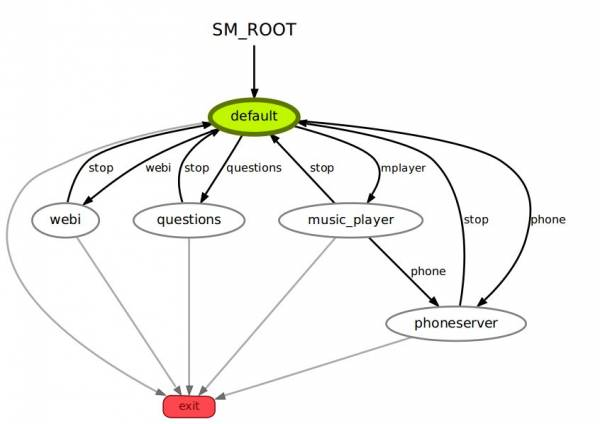
\includegraphics[height=5cm]{imgs/1_introduction/smach.jpg}
	\caption{Captura de SMACH viewer.}
	\label{fig:smach}
\end{figure}

Actualmente, herramientas similares a estas que acabamos de describir están siendo ampliamente utilizadas en la programación de Inteligencia Artificial (IA), especialmente para adversarios en los videojuegos. Vemos con esto que estas herramientas no tienen por qué estar ligadas necesariamente a robots, si no que tienen más aplicaciones. \\

\begin{figure}[htbp!]
	\centering
	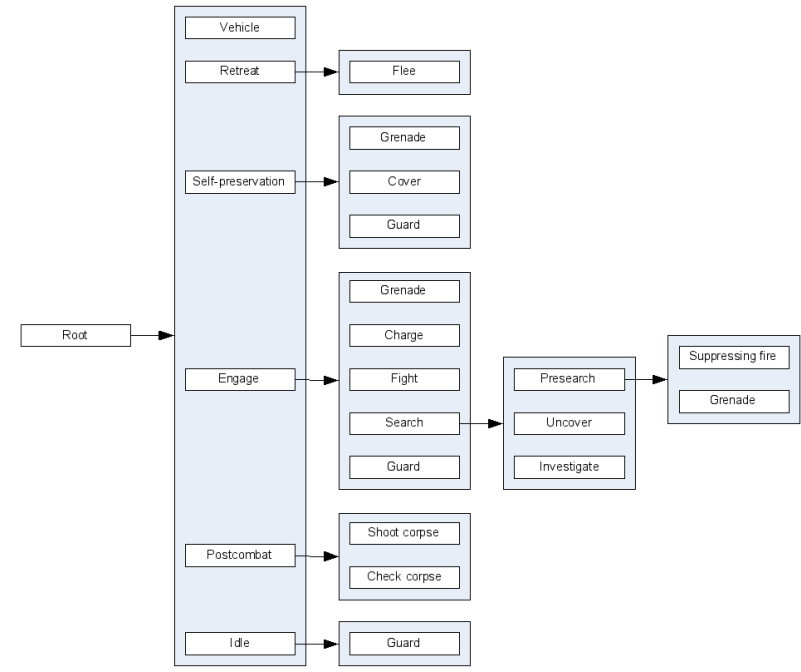
\includegraphics[width=11.5cm]{imgs/1_introduction/halo_2.png}
	\caption{Ejemplo de autómata del videojuego Halo 2.}
	\label{fig:halo2}
\end{figure}

En la figura \ref{fig:halo2} se puede observar un comportamiento programado mediante un autómata finito y jerárquico, similar a los que hemos estado describiendo. Este ejemplo proviene del videojuego Halo 2, y representa la inteligencia de los jugadores automáticos. Cada acción del primer nivel despliega uno o más niveles, especializando con cada paso las acciones a ejecutar. \\

\enspace
Con estos temas principales en los que hemos centrado esta sección, las plataformas, los LPV, y el uso de autómatas finitos para la programación del comportamiento, hemos introducido los dos pilares fundamentales sobre los que se apoya nuestra herramienta, VisualHFSM, de la que hablaremos a continuación.

%%%%%%%%%%%%%%% VisualHFSM %%%%%%%%%%%%%%%
\section{VisualHFSM}
Para terminar con este capítulo de introducción, vamos a hablar a continuación de la herramienta de la plataforma JdeRobot en la que se centra este TFG: VisualHFSM (\textit{Visual Hierarchy Finit State Machine}). VisualHFSM es una herramienta que combina ventajas de los LPV y del uso de las máquinas de estados finitos jerárquicos para desarrollar el comportamiento de robots de forma sencilla, haciendo que el desarrollador tenga que preocuparse de programar sólo el código imprescindible. Para crear un autómata bastará con \textit{dibujar} los estados y transiciones que van a definir su comportamiento en la ventana del editor gráfico. Esto definirá el flujo de control del autómata, y, a continuación, se puede añadir el código que se desee que se ejecute en cada estado o en las transiciones. \\

Se puede usar el editor gráfico además para generar el archivo de configuración necesario para conectar el componente creado con sus interfaces ICE (lo explicaremos más adelante), si se desean incluir librerías adicionales, e incluso compilar el autómata mediante CMake\footnote{\url{https://cmake.org/}}, también generado automáticamente. El proyecto se guardará utilizando un archivo XML, en el que se escribirán todos los datos necesarios para reconstruirlo a la hora de abrirlo para seguir trabajando con él. Todo esto se materializa en código que el autómata ejecuta en rápidas iteraciones periódicas, comprobando en cada iteración en que estado se encuentra, si se debe transitar o no a otro estado, y ejecutando el código del estado correspondiente. La velocidad con la que estas iteraciones se producen  también puede modificarse mediante VisualHFSM. \\

Es importante tener en cuenta que esta no es una herramienta nueva creada en este TFG, sino que proviene de la evolución que ha ido sufriendo a lo largo de los años durante sus diferentes versiones. Es un proyecto complejo y potente que ha sufrido un largo proceso de maduración para llegar a su estado actual. \\

La primera versión de esta herramienta fue desarrollada por Carlos Iván\footnote{\url{http://jderobot.org/Cmartin-pfc-itis}} en su TFG\cite{martin2010herramienta} en el año 2010. Todavía no recibió el nombre de VisualHFSM y fue el primer acercamiento desarrollado en la Universidad Rey Juan Carlos dentro de la plataforma JdeRobot, siendo compatible con su versión 4.3. Permitía la programación de robots mediante autómatas mononivel que funcionaban sobre el componente básico de dicha versión. Contaba con todo lo esencial para diseñar los autómatas de estado finito de manera visual y autogenerar código en C, incluyendo una versión inicial de la GUI y cómo guardar el proyecto en un archivo XML. \\

La siguiente versión de esta herramienta la realizó David Yunta\footnote{\url{http://jderobot.org/Dyunta-pfc-itis}} en el año 2011\cite{yunta2012herramienta, paperDavidYunta}], y su principal mejora introducida fue la migración de la aplicación a a nueva versión de JdeRobot, la 5.0. Esta versión de VisualHFSM nos permitía seguir desarrollando autómatas mononivel y generaba el código inspirado en el componente \textit{Introrob}, también perteneciente a la misma plataforma. Contaba con una interfaz gráfica nueva y con una gran mejora en los componentes generados, dado que éstos incluían una GUI en tiempo de ejecución. Esta GUI mostraba los estados por los que el robot iba transitando a medida que ejecutaba su comportamiento programado. Esto era una poderosa característica que facilitaba mucho las tareas de depuración del código, permitiendo controlar en todo momento si el robot se estaba comportando como el desarrollador esperaba que lo hiciese. Además, el código que generaba la aplicación era C++. \\

Visual HFSM 3.0\cite{salamanques2012} fue realizada por Rubén Salamanqués\footnote{\url{http://jderobot.org/Rubensb-pfc-itis}} en el año 2012. Con esta versión Rubén dotó a la herramienta de mayor poder, al hacer posible que trabajase con autómatas jerárquicos, permitiendo que dentro de un estado pudiese haber subautómatas. Con esto se consiguió que la herramienta sirviese para programar comportamientos más complejos de una manera más sencilla. La única pega que esta mejora tuvo fue que supuso la pérdida de la GUI en tiempo de ejecución, pues esta GUI sólo estaba planteada para soportar autómatas mononivel. El código que generaba también era C++ y seguía siendo compatible con la versión de JdeRobot 5.0. \\

La cuarta y última versión hasta la fecha, VisualHFSM 4.0\cite{borja2014, menendezprogramming}, fue desarrollada por Borja Menéndez\footnote{\url{http://jderobot.org/Bmenendez-tfm}}. Las principales mejoras son que incluyó ejemplos usando el robot \textit{Nao}, mientras que hasta ahora sólo se había podido usar VisualHFSM con el robot \textit{Pioneer}. Además renovó la GUI, haciendo que el canvas para dibujar el autómata fuese más espacioso y añadió el \textit{Tree View}, donde se podía ver la representación textual del autómata entero, mostrando sus distintos subniveles debajo de su nodo padre para ver todos los estados del autómata, algo muy útil para trabajar con autómatas multinivel. Sin embargo, la herramienta seguía sin recuperar la GUI en ejecución.

\begin{figure}[htbp]
	\begin{subfigure}{0.4\textwidth}
	\centering
	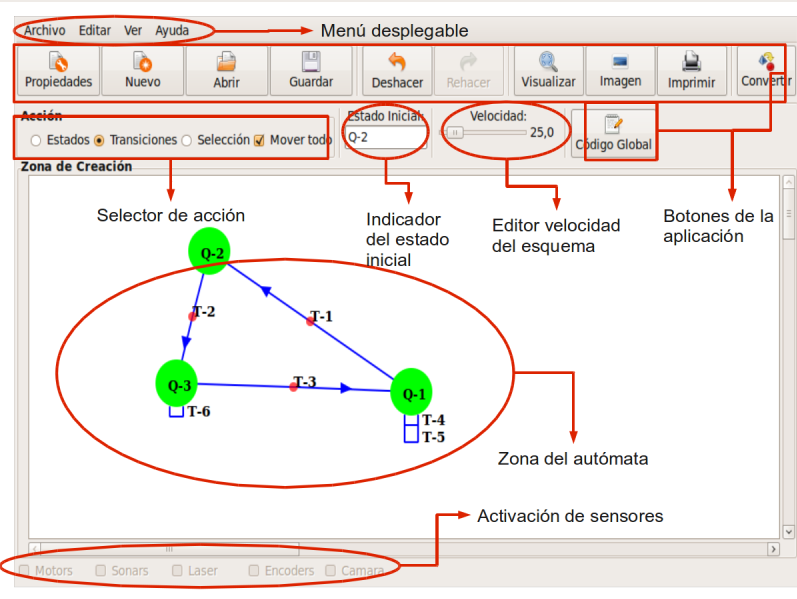
\includegraphics[height=4cm]{imgs/1_introduction/visualHFSM1.png}
	\caption{VisualHFSM 1.0}
	\label{fig:visualHFSM1}
	\end{subfigure}
	\hfill
	\begin{subfigure}{0.4\textwidth}
	\centering
	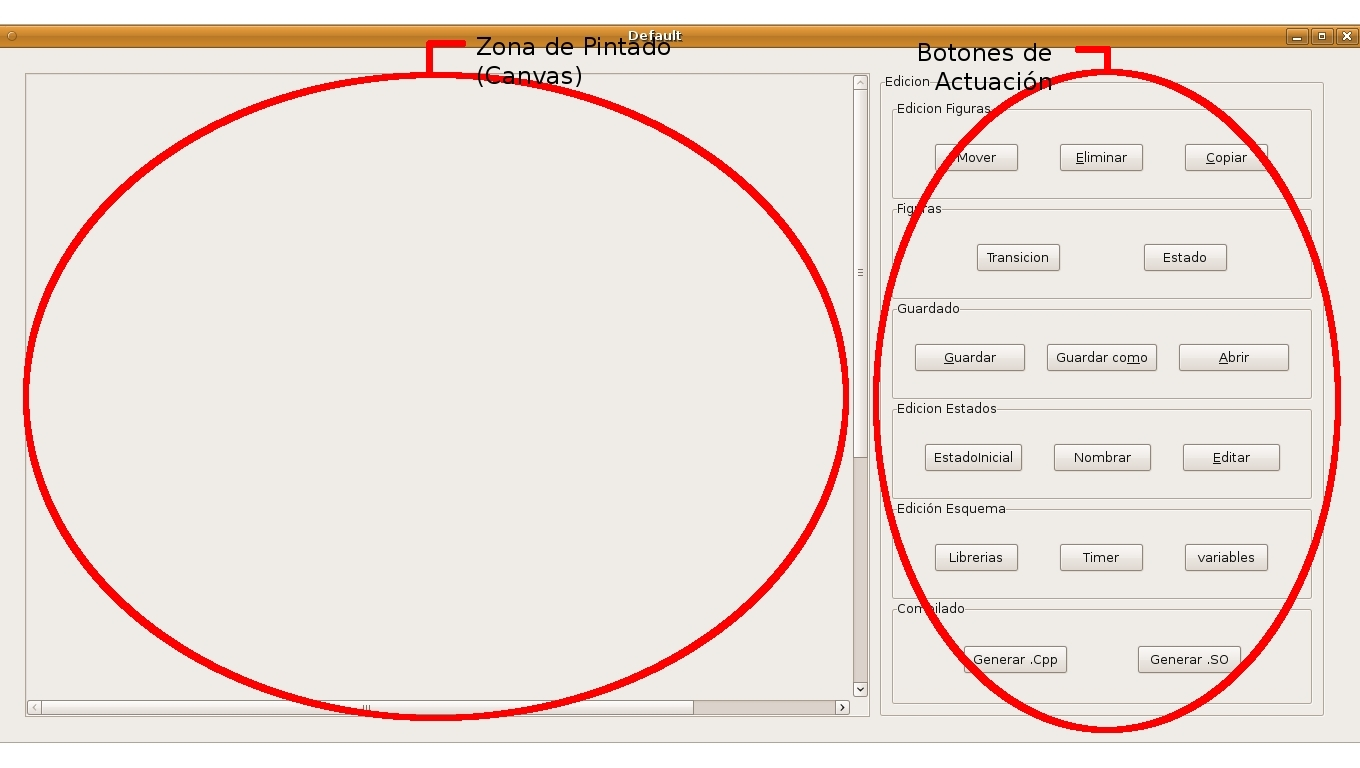
\includegraphics[height=4cm]{imgs/1_introduction/visualHFSM2.jpg}
	\caption{VisualHFSM 2.0}
	\label{fig:visualHFSM2}
	\end{subfigure}
	\hfill
	\begin{subfigure}{0.4\textwidth}
	\centering
	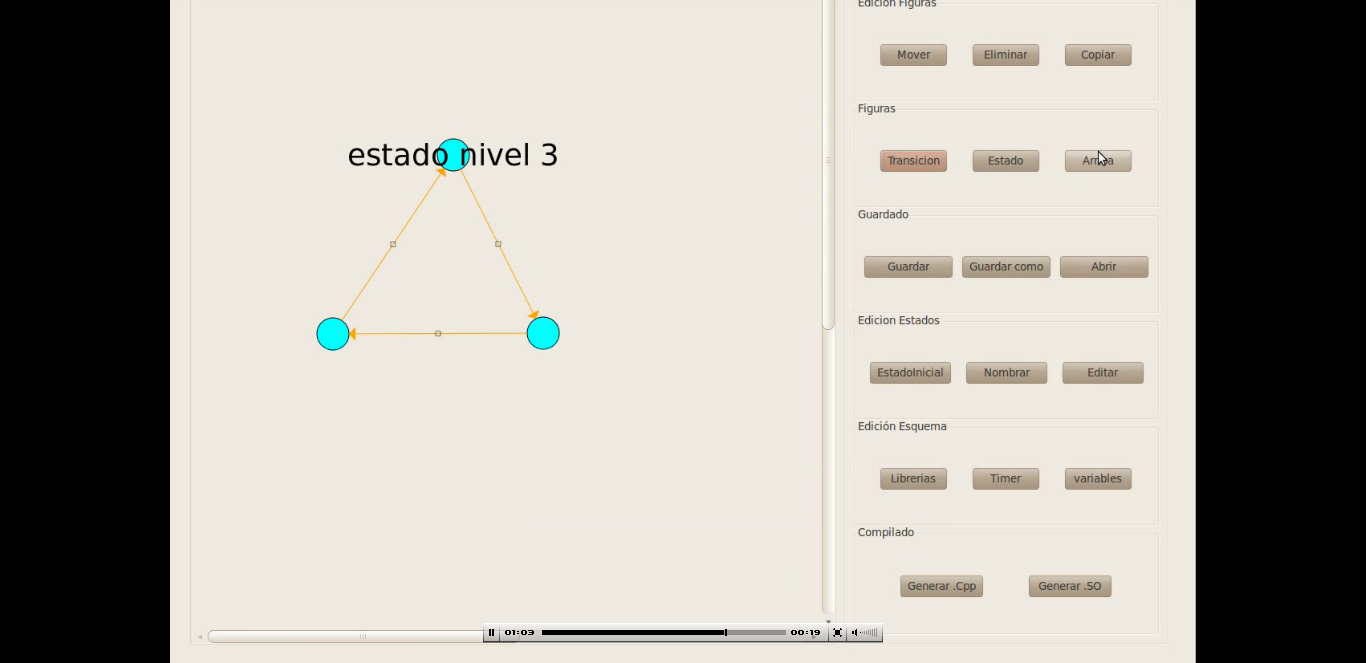
\includegraphics[height=4cm]{imgs/1_introduction/visualhfsm3.png}
	\caption{VisualHFSM 3.0}
	\label{fig:visualHFSM3}
	\end{subfigure}
	\hfill
	\begin{subfigure}{0.4\textwidth}
	\centering
	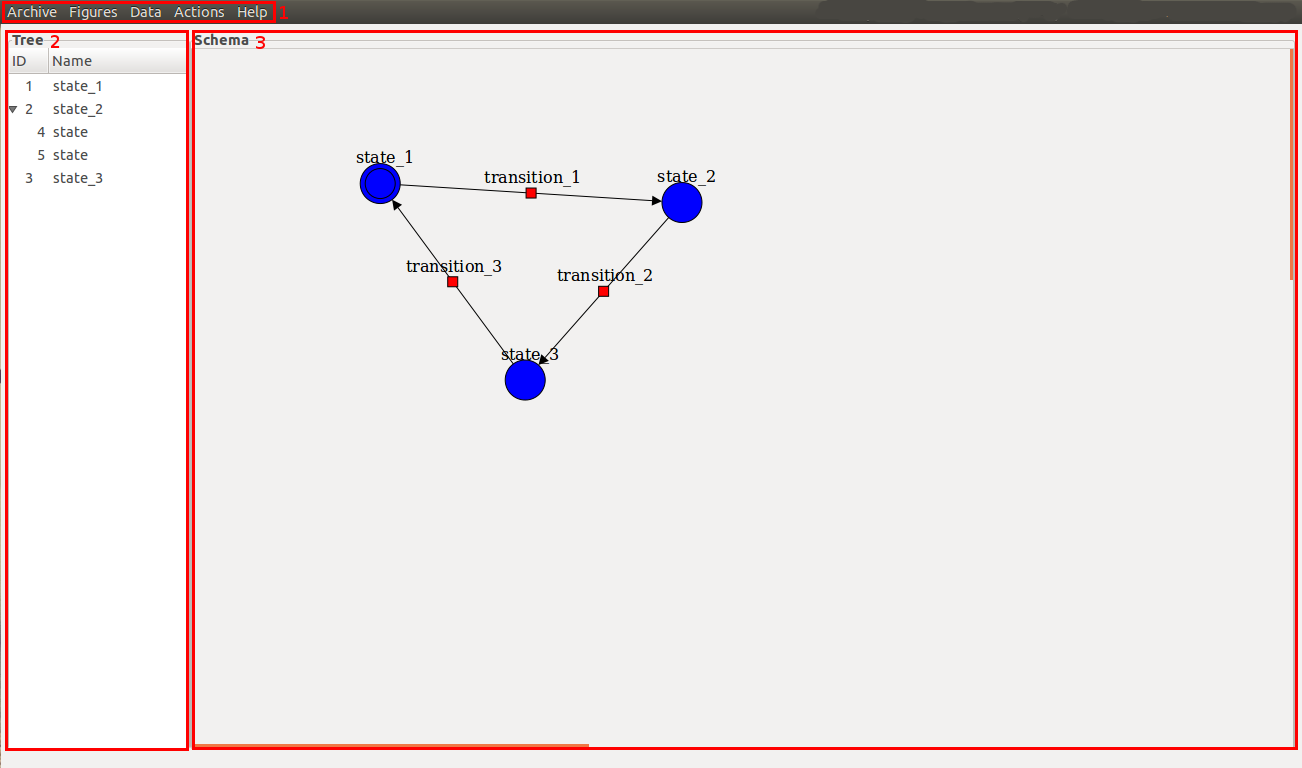
\includegraphics[height=4cm]{imgs/1_introduction/visualHFSM4.png}
	\caption{VisualHFSM 4.0}
	\label{fig:visualHFSM4}
	\end{subfigure}
\caption{Evolución de la GUI a lo largo de las distintas versiones de VisualHFSM}
\label{fig:visualHFSMGUIs}
\end{figure}

A la hora de ejecutar los autómatas creados por esta herramienta hay que tener en cuenta que, desde que soportan jerarquía, es un código \textit{multi-hilo}, dado que cada subautómata supone un hilo de ejecución distinto. El componente generado está preparado para soportar esto, pero si el código que se inyecta en los estados y transiciones es sensible a las condiciones de carrera, el programador deberá ser consciente de esta situación y utilizar las medidas necesarias para solventarlo. Aunque, cómo acabamos de explicar, hay un hilo de ejecución por cada subautómata, no todos están activos a la vez. Cada hilo sólo está ejecutando el código de su estado activo y comprobando si tiene que transitar a otros estados cuando su padre está activo. En caso contrario, el hilo estará esperando a que su padre se active sin hacer nada. \\

En cuánto al hilo de ejecución que sigue cada subautómata, la idea es sencilla. En un primer lugar entra en un \textit{switch-case} de control. Aquí cada subautómata se encarga de evaluar si su padre está activo (en caso de tenerlo), y de ser así, comprueba cuál es su estado activo, y si se cumple alguna de las condiciones necesarias para que se active una de sus transiciones. Si éste es el caso, se ejecutará el código de la transición (en caso de haberlo), y se pondrá como estado activo de este subautómata el nuevo estado. En caso de que no sea necesario realizar ninguna transición, el estado activo seguirá siendo el mismo. A continuación, hay un \textit{switch-case} de acción. Ahora, si el padre está activo, se comprueba cuál es el estado actual y se ejecuta su código. Todo esto se encuentra dentro de un bucle infinito, y se repite periódicamente en función de la frecuencia que el programador haya establecido mediante el editor.

\vspace{1.5cm}
En el segundo capítulo describiremos los objetivos concretos y fijaremos los requisitos que debe cumplir esta nueva versión de VisualHFSM a desarrollar en este proyecto. En el capítulo de infraestructura se analizarán en detalle las herramientas software que se han empleado. En el cuarto capítulo describiremos de forma detallada las soluciones que se han programado para conseguir los objetivos propuestos. En el siguiente, comprobaremos experimentalmente el funcionamiento de la estructura conseguida, montando distintos comportamientos para drones, todos generados con VisualHFSM 5.0. Por último, esta memoria terminará describiendo las conclusiones a las que hemos llegado, y las posibles líneas futuras de trabajo a partir de este proyecto.